\documentclass[a4paper]{G2-105}
\usepackage[utf8]{luainputenc}

\usepackage[dvipsnames]{xcolor}
\usepackage{listings}

\graphicspath{{figures/}}

\newcommand{\CommonSoftwareRequirements}{
\begin{itemize}
\item git;
\item nvm;
\item Node.js~v6.0.0;
\item npm~v3.8.6;
\item MongoDB~v2.6.12;
\item Stardog~v4.1.
\end{itemize}
}

\newcommand{\CommonBrowserRequirements}{
\begin{itemize}
\item Google Chrome~30.0;
\item Mozilla Firefox~25.0;
\item Apple Safari~6;
\item Microsoft Internet Explorer~9.
\end{itemize}
}

\newcommand{\CommonSystemRequirements}{
\begin{itemize}
\item процессор с тактовой частотой не ниже 2.7 ГГц;
\item объем оперативной памяти не ниже 512 Мб;
\item объем жесткого диска не ниже 10 Гб.
\end{itemize}
}

\newcommand{\CommonClientRequirements}{
\begin{itemize}
\item процессор с тактовой частотой не ниже 1600 МГц;
\item объем оперативной памяти не ниже 1024 Мб;
\item объем жесткого диска не ниже 20 Гб;
\item монитор с диагональю не менее 15 дюймов;
\item манипулятор типа «мышь», клавиатура.
\end{itemize}
}

\newcommand{\CommonGoal}{повышение качества принимаемых решений по управлению отходами на предприятии за счет организации интеллектуальной поддержки процесса принятия решений на основе онтологической модели представления знаний и логического вывода на онтологии}


\newcommand{\CommonGoalCap}{Повышение качества принимаемых решений по управлению отходами на предприятии за счет организации интеллектуальной поддержки процесса принятия решений на основе онтологической модели представления знаний и логического вывода на онтологии}

\newcommand{\CommonTasks}{
\begin{itemize}
\item провести анализ процесса и специфики управления отходами на предприятии с целью построения информационно-логической модели предметной области и формирования требований к модели представления знаний;
\item разработать концепцию поддержки принятия решений по управлению отходами предприятия на основе онтологической модели представления знаний и логического вывода на онтологии;
\item разработать онтологическую модель предметной области и алгоритм генерации стратегии управления отходами предприятия на основе логического вывода на онтологии;
\item разработать и протестировать интеллектуальную систему поддержки принятия решений по управлению отходами на основе предложенных модели и алгоритма.
\end{itemize}
}

\def\CommonOntologyModelFormula{O = \left<C,~R,~F\right >}
\def\CommonOntologyModelDescription{\begin{VSTUFormulaWhereList}
\item $C$~--- конечное множество понятий (концептов) предметной области, которую представляет онтология О;
\item $R$~--- конечное множество отношений между концептами;
\item $F$~--- конечное множество функций интерпретации, заданных на концептах и/или отношениях онтологии О.
\end{VSTUFormulaWhereList}
}

\newcommand{\CommonTprFormulaCompact}{$DS = \left<S,~A,~C,~M,~P,~R\right>$, где $S$~-- описание ситуации принятия решений, состоящее из множества численных и качественных параметров: $S = \left\{P_{q1},~P_{q2},~...,~P_{qn1},~P_{qn2}\right\}$; $A$~-- множество альтернатив, каждая из которых состоит из множества управляющих воздействий: $A = \left\{A_{c1},~A_{c2},~...,\right\}$; $C$~-- множество критериев, в виде качественных оценок ситуации с точки зрения предприятия; $M$~-- модель, позволяющая для каждой альтернативы рассчитать вектор критериев; $P$~-- система предпочтений для каждого из критериев; $R$~-- решающее правило выбора альтернативы}

\def\CommonTprFormula{DS = \left<S,~A,~C,~M,~P,~R\right>}
\def\CommonTprDescription{\begin{VSTUFormulaWhereList}
\item $S$~--- описание ситуации принятия решений, состоящее из множества численных и качественных параметров, $S = \left\{P_{q1},~P_{q2},~...,~P_{qn1},~P_{qn2}~\right\}$;
\item $A$~--- множество альтернатив, каждая из которых состоит из множества управляющих воздействий: $A = \left\{A_{c1},~A_{c2},~...,~A_{cm}\right\}$;
\item $C$~--- множество критериев, в виде качественных оценок ситуации с точки зрения предприятия;
\item $M$~--- модель, позволяющая для каждой альтернативы рассчитать вектор критериев;
\item $P$~--- система предпочтений для каждого из критериев;
\item $R$~--- решающее правило выбора альтернативы.
\end{VSTUFormulaWhereList}
}

\newcommand{\CommonMetaontologyModels}{
\begin{itemize}
\item онтология отходов, описывающая их свойства и классы опасности, а также негативное влияние, которые они оказывают на окружающую среду;
\item онтология субъектов, взаимодействующих с отходами (предприятие, полигон и т. д.);
\item онтология методов управления отходами, описывающая методы (переработка, утилизации, транспортировки и т.д.) и их стоимость, экологический вред, который также должен оплачиваться субъектом согласно закону РФ.
\end{itemize}
}

\newcommand{\CommonMetaontologyFormulaCompact}{$M = \left<O_{M},~C_{M},~Inst_{M},~R_{M},~I_{M}\right>$, 

где $M$ -- метаонтологическая модель предметной области; $O_{M} = \left\{O_{W},~O_{M},~O_{S}\right\}$~-- множество онтологических моделей, объединенных в метаонтологию, $O_{W}$~-- онтология отходов, $O_{M}$~-- онтология методов управления отходами,  $O_{S}$~-- онтология субъектов управления отходами; $C_{M}$~-- конечное множество концептов, $C_{M} = \varnothing$; $Inst_{M}$~-- конечное множество экземпляров классов, $Inst_{M} = \varnothing$; $R_{M} = \left\{has,~uses,~includes\right\}$~-- конечное множество отношений метаонтологии; $I_{M}$~-- множество правил интерпретации и ограничений, $I_{M} = \varnothing$}

\def\CommonMetaontologyFormula{M = \left<O_{M},~C_{M},~Inst_{M},~R_{M},~I_{M}\right>}
\def\CommonMetaontologyDescription{\begin{VSTUFormulaWhereList}
\item $M$~--- метаонтологическая модель предметной области;
\item $O_{M}$~--- множество онтологических моделей, объединенных в метаонтологию: $O_{M} = \left\{O_{W},~O_{M},~O_{S}\right\}$, где $O_{W}$~-- онтология отходов, $O_{M}$~-- онтология методов управления отходами,  $O_{S}$~-- онтология субъектов управления отходами;
\item $C_{M}$~--- конечное множество концептов, $C_{M} = \varnothing$;
\item $Inst_{M}$~--- конечное множество экземпляров классов, $Inst_{M} = \varnothing$;
\item $R_{M}$~--- конечное множество отношений метаонтологии $M$: $R = \left\{r_{M1},~r_{M2},~r_{M3}\right\}$, где $r_{M1}$~-- отношение has «имеет», $r_{M2}$~-- отношение uses «использует», $r_{M3}$~-- отношение includes «включает»;
\item $I_{M}$~--- множество правил интерпретации и ограничений, $I_{M} = \varnothing$.
\end{VSTUFormulaWhereList}
}

\newcommand{\CommonWasteOntologyCompact}{$O_{W} = \left<C_{W},~Inst_{W},~R_{W},~I_{W}\right>$, 

где $C_{W}$~-- конечное множество концептов онтологии отходов, $C_{W} = \left\{C_{W1},~...,~C_{W26}\right\}$; $Inst_{W}$~-- множество экземпляров классов онтологии отходов, $Inst_{W} = \left\{i_{W1},~i_{W2},~...,~i_{Wj},~...,~i_{Wn}\right\}$; $R_{W}$~-- конечное множество отношений онтологии отходов: $R_{W} = \left\{r_{W1},~...,~r_{W8}\right\}$, где $r_{W1}$~-- отношение $hasHazard$, $r_{W2}$~-- отношение $hasAggregateState$, $r_{W3}$~-- relation $hasOrigin$, $r_{W4}$~-- отношение $hasAmount$, $r_{W5}$~-- отношение $hasTitle$, $r_{W6}$~-- отношение $hasEcolTax$, $r_{W7}$~-- отношение $is$, $r_{W8}$~-- отношение $is-a$; $I_{W}$~-- множество правил}

\def\CommonWasteOntologyFormula{O_{W} = \left<C_{W},~Inst_{W},~R_{W},~I_{W}\right>}
\def\CommonWasteOntologyDescription{\begin{VSTUFormulaWhereList}
\item $C_{W}$~--- конечное множество концептов онтологии отходов: $C_{W} = \left\{C_{W1},~...,~C_{W26}\right\}$;
\item $Inst_{W}$~--- множество экземпляров классов онтологии отходов: $Inst_{W} = \left\{i_{W1},~i_{W2},~...,~i_{Wj},~...,~i_{Wn}\right\}$;
\item $R_{W}$~--- конечное множество отношений онтологии отходов: $R_{W} = \left\{r_{W1},~...,~r_{W8}\right \}$, где $r_{W1}$~-- отношение $hasHazard$, $r_{W2}$~-- отношение $hasAggregateState$, $r_{W3}$~-- relation $hasOrigin$, $r_{W4}$~-- отношение $hasAmount$, $r_{W5}$~-- отношение $hasTitle$, $r_{W6}$~-- отношение $hasEcolTax$, $r_{W7}$~-- отношение $is$, $r_{W8}$~-- отношение $is-a$;
\item $I_{W}$~--- множество правил и ограничений (методика их добавления рассмотрена далее).
\end{VSTUFormulaWhereList}
}

\newcommand{\CommonMethodOntologyCompact}{$O_{M} = \left<C_{M},~Inst_{M},~R_{M},~I_{M}~\right>$, где $C_{M}$~-- конечное множество концептов онтологии методов управления отходами, $C_{M} = \left\{C_{M1},~...,~C_{M6}\right\}$; $Inst_{M}$~-- множество экземпляров классов онтологии методов управления отходами, $Inst_{M} = \left\{i_{M1},~i_{M2},~...,~i_{Mj},~...,~i_{Mn}\right\}$; $R_{M}$~-- множество отношений онтологии методов управления отходами, $R_{M} = \left\{r_{M1},~...,~r_{M8}\right\}$, где $r_{M1}$~-- отношение $is$, $r_{M2}$~-- отношение $hasTitle$, $r_{M3}$~-- отношение $hasMethod$, $r_{M4}$~-- отношение $processedBy$, $r_{M5}$~-- отношение $hasHarmfulEffect$, $r_{M6}$~-- отношение $hasCostOnDistance$, $r_{M7}$~-- отношение $hasCostOnWeight$, $r_{M8}$~-- отношение $hasCostByService$; $I_{M}$~-- множество правил интерпретации и ограничений, $I_{M} = \varnothing$}

\def\CommonMethodOntologyFormula{O_{M} = \left<C_{M},~Inst_{M},~R_{M},~I_{M}\right>}
\def\CommonMethodOntologyDescription{\begin{VSTUFormulaWhereList}
\item $C_{M}$~--- конечное множество концептов онтологии методов управления отходами: $C_{M} = \left\{C_{M1},~...,~C_{M6}\right\}$;
\item $Inst_{M}$~--- множество экземпляров классов онтологии методов управления отходами: $Inst_{M} = \left\{i_{M1},~i_{M2},~...,~i_{Mj},~...,~i_{Mn}\right\}$;
\item $R_{M}$~--- множество отношений онтологии методов управления отходами: $R_{M} = \left\{r_{M1},~...,~r_{M8}\right\}$, где $r_{M1}$~-- отношение $is$, $r_{M2}$~-- отношение $hasTitle$, $r_{M3}$~-- отношение $hasMethod$, $r_{M4}$~-- отношение $processedBy$, $r_{M5}$~-- отношение $hasHarmfulEffect$, $r_{M6}$~-- отношение $hasCostOnDistance$, $r_{M7}$~-- отношение $hasCostOnWeight$, $r_{M8}$~-- отношение $hasCostByService$;
\item $I_{M}$~--- множество правил интерпретации и ограничений, $I_{M} = \varnothing$.
\end{VSTUFormulaWhereList}
}

\newcommand{\CommonSubjectOntologyCompact}{$O_{S} = \left<C_{S},~Inst_{S},~R_{S},~I_{S}\right>$, где $C_{S}$~-- конечное множество концептов субъектов управления отходами, $C_{S} = \left\{C_{S1},~...,~C_{S6}\right\}$; $Inst_{S}$~-- множество экземпляров классов онтологии субъектов управления отходами, $Inst_{S} = \left\{i_{S1},~i_{S2},~...,~i_{Sj},~...,~i_{Sn}\right\}$; $R_{S}$~-- множество отношений онтологии субъектов управления отходами, $R_{S} = \left\{r_{S1},~...,~r_{S9}\right\}$, $r_{S1}$~-- отношение is, $r_{S2}$~-- отношение locatedIn, $r_{S3}$~-- отношение hasCoordinates, $r_{S4}$~-- отношение hasEcolOfGround, $r_{S5}$~-- отношение hasTitle, $r_{S6}$~-- отношение hasWaste, $r_{S7}$~-- отношение hasMethod, $r_{S8}$~-- отношение hasBudget, $r_{S9}$~-- отношение hasEcolOfAir; $I_{S}$~-- множество правил интерпретации и ограничений, $I_{S} = \varnothing$}

\def\CommonSubjectOntologyFormula{O_{S} = \left<C_{S},~Inst_{S},~R_{S},~I_{S}\right>}
\def\CommonSubjectOntologyDescription{\begin{VSTUFormulaWhereList}
\item $C_{S}$~--- конечное множество концептов субъектов управления отходами: $C_{S} = \left\{C_{S1},~...,~C_{S6}\right\}$;
\item $Inst_{S}$~--- множество экземпляров классов онтологии субъектов управления отходами: $Inst_{S} = \left\{i_{S1},~i_{S2},~...,~i_{Sj},~...,~i_{Sn}\right\}$;
\item $R_{S}$~--- множество отношений онтологии субъектов управления отходами: $R_{S} = \left\{r_{S1},~...,~r_{S9}\right\}$, где $r_{S1}$~-- отношение is, $r_{S2}$~-- отношение locatedIn, $r_{S3}$~-- отношение hasCoordinates, $r_{S4}$~-- отношение hasEcolOfGround, $r_{S5}$~-- отношение hasTitle, $r_{S6}$~-- отношение hasWaste, $r_{S7}$~-- отношение hasMethod, $r_{S8}$~-- отношение hasBudget, $r_{S9}$~-- отношение hasEcolOfAir;
\item $I_{S}$~--- множество правил интерпретации и ограничений, $I_{S} = \varnothing$.
\end{VSTUFormulaWhereList}
}

\def\CommonTaskGivenFormula{s = \left<Coord_{s},~L_{s},~B_{s},~W_{s},~M_{s}\right>}
\def\CommonTaskGivenDescription{\begin{VSTUFormulaWhereList}
\item $s$~--- предприятие, являющиеся экземпляром класа $Subject$ онтологии $O_{S}$;
\item $Coord_{s}$~--- координаты предприятия, строка;
\item $L_{s}$~--- локация предприятия, определяющая город, регион и др.: $L_{s} = \left\{l_{1},~l_{2},~...,~l_{i},~...,~l_{n}\right\}$, где $l_{i}$~-- экземпляр класса $Subject$ онтологии $O_{S}$;
\item $B_{s}$~--- бюджет предприятия, число;
\item $W_{s}$~--- отходы предприятия, сгрупированные по методу управления отходами $W_{s} = \left\{W_{1},~W_{2},~...,~W_{i},~...,~W_{n}\right\}$, где $W_{i}$~-- подмножество отходов, объединенных общим признаком -- метод управления $m_{i}$, $W_{i} = \left\{w_{i1},~w_{i2},~...,~w_{ij}\right\}$, где $w_{ij}$~-- экземпляр класса $Waste$ онтологии $O_{W}$;
\item $M_{s}$~--- методы управления отходами предприятия: $M_{s} = \left\{m_{1},~m_{2},~...,~m_{i},~...,~m_{n}\right\}$, где $m_{i}$~--- экземпляр класса $Method$ онтологии $O_{M}$. 
\end{VSTUFormulaWhereList}
}

\def\CommonFormalOntologyTask{M|_{min(ecol, econ)} = \{M_{1},~M_{2}~...,~M_{k}\} : k = |W_{s}|.}
\def\CommonFormalOntologySolution{St_{s} = \{\left<W_{1},~M_{1}\right>,~\left<W_{2},~M_{2}\right>,~...,~\left<W_{n},~M_{n}\right>\}.}

\newcommand{\CommonScientificNovations}{
\begin{itemize}
\item Разработана интегрированная онтологическая модель представления знаний по управлению отходами предприятия, которая отличается от известных возможностью описания данных и знаний об объектах и субъектах процесса управления отходами на общем домене концептов, а также позволяет реализовывать логический вывод на онтологии на основе семантических запросов.
\item Разработан алгоритм генерации эффективной стратегии управления отходами на основе логического вывода на онтологической модели с использованием семантических запросов.
\end{itemize}
}

\newcommand{\CommonPracticalValue}{
\begin{itemize}
\item Разработанные в диссертационной работе модели и алгоритм позволяют производить генерацию эффективной стратегии управления отходами на предприятии. Реализованная система поддержки принятия решений включает в себя модуль генерации стратегии управления отходами на предприятии, а также онтологическую базу знаний отходов, методов и субъектов управления отходами. Разработана методика создания и расширения онтологической базы знаний предметной области, что позволяет применять данную систему, учитывая особенности различных субъектов управления отходами и видов отходов. В результате повышается качество принимаемых решений в области обращения с отходами на предприятии при использовании предложенной системой стратегии управления отходами.
\item Реализованная система поддержки принятия решений прошла аппробацию в учреждении ГБУЗ «Николаевское ЦРБ» в процессе обращения с отходами. 
\item Работа выполнена при поддержке РФФИ в рамках проекта №15-07-03541 «Интеллектуальная поддержка принятия решений по управлению сложными системами на основе интеграции различных типов рассуждений на знаниях, представленных онтологической моделью».
\end{itemize}
}

\newcommand{\CommonResults}{
\begin{itemize}
\item Проведен анализ процессов управления отходами на предприятии; информационных систем, используемых при принятии решений по управлению отходами; обзор моделей и методов, используемых при поддержке принятия решений по управлению отходами. Основным недостатком существующего процесса является сложность и трудоемкость процесса принятия верного решения экпертом в области управления отходами на предприятии. Построена информационно-логическая модель предметной области, включающая функциональную и объектную модели. Выявлены требования к модели представления знаний для описания объектов и субъектов процесса управления отходами на предприятии.
\item Разработана концепция поиска эффективной стратегии управления отходами на предприятии. Предложенная концепция предполагает создание автоматизированной системы для решения задачи генерации стратегии управления отходами, что позволяет сократить трудоемкость решения задачи и повысить обоснованность принимаемых решений, за счет применения моделей и методов искусственного интеллекта -- онтологической модели представления знаний и логического вывода на онтологиях.
\item Разработана интегрированная онтологическая модель представления знаний предметной области, состоящая из следующих компонентов, объединенных метаонтологией: (1) онтология отходов; (2) онтология методов управления отходами; (3) онтология субъектов управления отходами. Разработанная модель позволяет описывать объекты и субъекты процесса управления отходами на общем домене концептов и решать задачу поиска эффективной стратегии управления отходами посредством логического вывода на онтологии. Разработан алгоритм генерации эффективной стратегии управления отходами на предприятии на основе логического вывода на онтологической модели с использованием языка семантических запросов.
\item Разработана архитектура и реализована интеллектуальная система поддержки принятия решений для генерации эффективной стратегии управления отходами на предприятии на основе описанных моделей и алгоритма. Проведено тестирование системы и проверка соответствия полученой стратегии управления отходами с данными по учреждению ГБУЗ «Николаевское ЦРБ». Стратегия управления отходами, полученная в результате генерации системой, соответствует сформулированным критериям эффективности и соответствует выбранным методом управления отходами, примененным учреждением ГБУЗ «Николаевское ЦРБ». Данный результат позволяет сделать вывод об эффективности разработанных моделей и алгоритма.
\end{itemize}
}

\newcommand{\CommonKeywords}{Ключевые слова: управление отходами, поддержка принятия решений, метаонтология, OWL-DL, логический вывод на онтологии, RDF, SPARQL, интеллектуальная система поддержки принятия решений}
\newcommand{\CommonKeywordsEng}{Keywords: waste management, decision support, Metaontology, OWL-DL, inference logical consequences, RDF, SPARQL, Intelligent Decision Support System}

\newcommand{\CommonPublicationsVAK}{
\begin{enumerate}
\item Кульцова,~М.Б. Интеллектуальная поддержка принятия решений по управлению отходами на городских территориях на основе онтологической модели представления знаний~/ Кульцова~М.Б., Руднев~Р.Ю., Жукова~И.Г., Аникин~А.В.~//~Изв. ВолгГТУ. Серия «Актуальные проблемы управления, вычислительной техники и информатики в технических системах». Вып. 13~:~межвуз. сб. науч. ст.~/~ВолгГТУ.~--~Волгоград,~2015.~--~№ 13 (117).~-- C.~104-109.
\end{enumerate}
}

\newcommand{\CommonPublicationsOther}{
\begin{enumerate}
\setcounter{enumi}{1}

\item Руднев,~Р.Ю. Онтологический подход к поддержке принятия решений по управлению отходами на городских территориях~/~Руднев~Р.Ю., Кульцова~М.Б., Жукова~И.Г.~//~XII Международная научно-практическая конференция «Инновации на основе информационных и коммуникационных технологий» ИНФО-2015 (Сочи, 1-10 окт. 2015 г.)~:~сб. науч. ст.~--~Сочи, 2015.~--~С.~568-571.

\item Руднев,~Р.Ю. Концепция поддержки принятия решений по управлению отходами на городских территориях на основе онтологического и имитационного моделирования~/~Руднев~Р.Ю., Кульцова~М.Б.~//~XX региональная конференция молодых исследователей Волгоградской области (Волгоград, 10-13 нояб. 2015 г.)~:~тез. докл.~/~отв. ред. А.В. Навроцкий~;~Волгогр. гос. техн. ун-т [и др.].~--~Волгоград, 2016.~--~C.~143-144.

\item Kultsova~M. An ontology-based approach to intelligent support of decision making in waste management~/~Kultsova~M., Rudnev~R., Anikin~A., Zhukova~I.~//~CIT DS Creativity in Intelligent Technologies Data Science, The 7th International Conference on Information, Intelligence, Systems and Applications,~IISA2016,~Greece,~2016 (принята к публикации).

\end{enumerate}
}

\newcommand{\CommonPublications}{
\begin{enumerate}

\item [1] Кульцова,~М.Б. Интеллектуальная поддержка принятия решений по управлению отходами на городских территориях на основе онтологической модели представления знаний~/ Кульцова~М.Б., Руднев~Р.Ю., Жукова~И.Г., Аникин~А.В.~//~Изв. ВолгГТУ. Серия «Актуальные проблемы управления, вычислительной техники и информатики в технических системах». Вып. 13~:~межвуз. сб. науч. ст.~/~ВолгГТУ.~--~Волгоград,~2015.~--~№ 13 (117).~-- C.~104-109.

\item [2] Руднев,~Р.Ю. Онтологический подход к поддержке принятия решений по управлению отходами на городских территориях~/~Руднев~Р.Ю., Кульцова~М.Б., Жукова~И.Г.~//~XII Международная научно-практическая конференция «Инновации на основе информационных и коммуникационных технологий» ИНФО-2015 (Сочи, 1-10 окт. 2015 г.)~:~сб. науч. ст.~--~Сочи, 2015.~--~С.~568-571.

\item [3] Руднев,~Р.Ю. Концепция поддержки принятия решений по управлению отходами на городских территориях на основе онтологического и имитационного моделирования~/~Руднев~Р.Ю., Кульцова~М.Б.~//~XX региональная конференция молодых исследователей Волгоградской области (Волгоград, 10-13 нояб. 2015 г.)~:~тез. докл.~/~отв. ред. А.В. Навроцкий~;~Волгогр. гос. техн. ун-т [и др.].~--~Волгоград, 2016.~--~C.~143-144.

\item [4] Kultsova~M. An ontology-based approach to intelligent support of decision making in waste management~/~Kultsova~M., Rudnev~R., Anikin~A., Zhukova~I.~//~CIT DS Creativity in Intelligent Technologies Data Science, The 7th International Conference on Information, Intelligence, Systems and Applications,~IISA2016,~Greece,~2016.

\end{enumerate}
}

% Информация для генерации титульных листов, хедеров и футеров
\VSTUSetDocumentNumbersPrefix{}
\VSTUSetDocumentCode{МД-40-461-806-10.19-09.04.04-08-16}
\VSTUSetDocumentTypeDative{магистерской диссертации}
\VSTUSetDocumentTypeAccusative{магистерскую диссертацию}
\VSTUSetDocumentTypeEng{master's thesis}
\VSTUSetInitialData{задание, выданное научным руководителем кафедры ПОАС, утвержденное приказом ректора университета}
\VSTUSetOrder{1551--ст}{20}{октябрь}{2014}
\VSTUSetDeadline{01}{июня}
\VSTUSetFaculty{Электроники и вычислительной техники}
\VSTUSetDepartment{Программное обеспечение автоматизированных систем}
\VSTUSetDepartmentCode{10.19}
\VSTUSetDirection{09.04.04 Программная инженерия}
\VSTUSetHeadOfDepartment{Зав. кафедрой ПОАС}{д.т.н., проф.}{А. М. Дворянкин}{Дворянкин Александр Михайлович}
\VSTUSetDirector{доц. каф. ПОАС}{к.т.н.}{М. Б. Кульцова}{Кульцова Марина Борисовна}
\VSTUSetStandardsAdviser{ст. преп. каф. ПОАС}{}{О. Н. Ляпина}{Ляпина Ольга Николаевна}
\VSTUSetReviewer{доц. каф. САПР и ПК}{д.т.н., проф.}{Н. П. Садовникова}{Садовникова Наталья Петровна}
\VSTUSetStudent{ПРИН-2Н}{Р. Ю. Руднев}{Руднев Роман Юрьевич}{Руднева Романа Юрьевича}
\VSTUSetStudentFullNameEng{Roman Rudnev}
\VSTUSetTitle{Интеллектуальная система поддержки принятия  решений  по  управлению  отходами}
\VSTUSetTitleEng{Intelligent decision support system of waste management}

% Определние цветов
\definecolor{dimgray}{HTML}{696969}
\definecolor{silver}{HTML}{C0C0C0}
\definecolor{darkgray}{HTML}{A9A9A9}

% Определение стилей
\lstdefinestyle{appendix}{
xleftmargin=8mm,
captionpos=b,
basicstyle=\ttfamily\footnotesize,
breakatwhitespace=false, 
breaklines=true,
keepspaces=true,
showspaces=false,
showstringspaces=false,
showtabs=false,                  
tabsize=2,
frame=single,
numbers=left,
stepnumber=1,
numbersep=7pt,
numberstyle=\footnotesize\color{silver}
}

\lstdefinestyle{default}{
basicstyle=\ttfamily\small,
xleftmargin=8mm,
breakatwhitespace=false,         
breaklines=true,                 
captionpos=b,                    
keepspaces=true,
showspaces=false,                
showstringspaces=false,
showtabs=false,                  
tabsize=2,
}

% Определение поддержки формата Turtle
\lstdefinelanguage{ttl}{
sensitive=true,
morecomment=[l][\color{dimgray}]{@},
morecomment=[l][\itshape\color{darkgray}]{\#},
morestring=[b]",
morekeywords={rdf,rdfs,owl,xsd}
}


\begin{document}

%
\VSTUSetDocumentNumbersPrefix{Ж.1.}
\VSTUInitializeRDOperator
%

\abstract{Аннотация}

Документ представляет собой руководство оператора для интеллектуальной системы поддержки принятия решений по управлению отходами на основе онтологической модели представления знаний и логического вывода на онтологиях. Документ содержит описание функций системы, описание операций, аварийных ситуаций и рекомендации по работе с системой. 

Настоящее руководство распространяется исключительно на систему и не заменяет учебную, справочную литературу, руководства от производителя ОС и прочие источники информации, освещающие работу с графическим
пользовательским интерфейсом операционной системы.

Документ включает в себя страниц~---~\totalpages, рисунков~---~\totalfigures.

\CommonKeywords

\newpage

\tableofcontents

\newpage

\chapter{Общие сведения о программе}

\ttl

\section{Полное наименование системы и ее условное обозначение}

Полное наименование системы -- «Интеллектуальная система поддержки принятия решений по управлению отходами предприятия».

Далее используется сокращенное наименование -- система.

\section{Область применения}

Система предназначена для решения задачи поиска стратегии управления отходами на предприятии на основе онтологической модели представления знаний и логического вывода на онтологии.

Сгенерированная стратегия управления отходами используется экспертом в качестве рекомендации при принятии решении в области обращения с отходами на предприятии.

\section{Краткое описание возможностей}

В данной системе пользователь имеет возможность:
\begin{itemize}
\item просматривать каталоги отходов и способов управления отходами;
\item создавать и редактировать профиль предприятия, его отходы и способы управления отходами;
\item просматривать сгенерированную системой стратегию управления отходами предприятия.
\end{itemize}

\section{Уровень подготовки пользователя}

Перед началом работы в системе пользователь должен изучить данное руководство и ознакомиться с системой.

\chapter{Назначение и условия применения}

\ttl

\section{Виды деятельности, функции}

Главная функция системы -- генерация стратегии управления отходами предприятия.

К основным функциям системы относятся:
\begin{itemize}
\item отображение каталогов отходов и способов управления отходами;
\item создание и редактирование профиля предприятия, его отходов и способ управления отходами.
\end{itemize}

К вспомогательным функциям системы относятся:
\begin{itemize}
\item регистрация новых пользователей системы;
\item загрузка онтологий предметной области управления отходами через конфигурационный файл.
\end{itemize}

\section{Программные и аппаратные требования к системе}

Для функционирования системы на стороне клиента необходимо следующее техническое обеспечение:
\CommonClientRequirements

Рабочей средой клиентской части системы можеть быть любая ОС с установленным в ней браузером:
\CommonBrowserRequirements

\chapter{Подготовка к работе}

\ttl

\section{Состав дистрибутива}

Так как система представляет собой клиент-серверное приложение с легким клиентом, пользователю для работы достаточно установить браузер. Описание процесса установки серверной части указано в руководстве системного программиста.

\section{Запуск системы}

Запуск системы производится при помощи запуска браузера и перехода по адресу, сервера на котором установлена серверная часть системы.

\section{Проверка работоспособности системы}

Для проверки работоспособности системы необходимо войти в систему, затем перейти в профиль своего предприятия и щелкнуть на кнопку поиска стратегии. После некоторого времени, система должна выдать результат генерации стратегии управления отходами на основе начальных данных из онтологии.

\chapter{Описание операций}

\ttl

\section{Вход в систему}

\ttl

\subsection{Наименование операции}

Полное наименование операции «Вход в систему».

\subsection{Условия выполнения операции}

Операция выполняется только если пользователь еще не был аутентифицирован в системе.

\subsection{Основные действия}

Пользователь должен ввести свой логин и пароль, затем нажать кнопку «Войти». В случаи если пользователь ввел корректные данные для входа, то он будет перенаправлен на страницу предприятий, иначе появится сообщение об ошибке.

На рисунке~\ref{fig:screen_login} представлена форма входа в систему.

\begin{figure}[H]
\centering
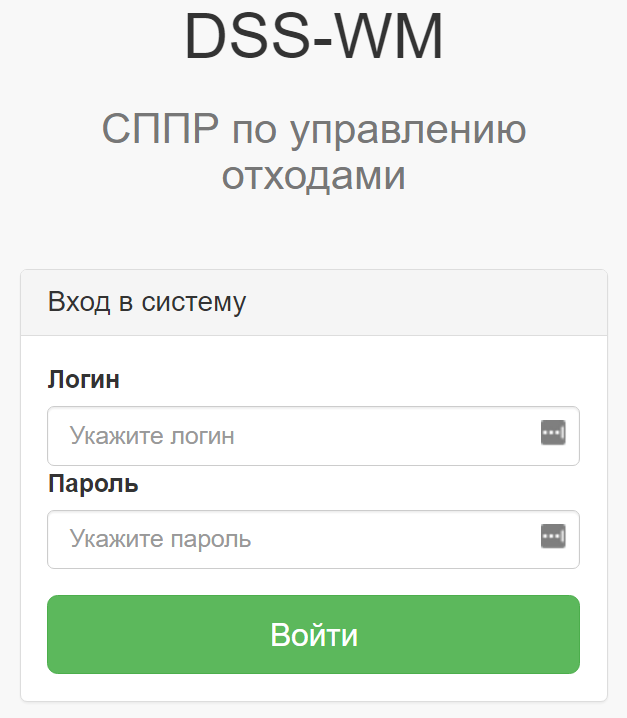
\includegraphics[scale=0.5]{screen_login}
\caption{Вход в систему}
\label{fig:screen_login}
\end{figure}

\section{Просмотр профиля предприятия}

\ttl

\subsection{Наименование операции}

Полное наименование операции «Просмотр профиля предприятия».

\subsection{Условия выполнения операции}

Операция выполняется только если пользователь имеет доступные ему предприятия.

\subsection{Основные действия}

Необходимо в меню выбрать пункт -- «Предприятие». Затем щелкнуть на иконку «глаз» в столбце действия таблицы (см. рисунок~\ref{fig:screen_companies}). После чего пользователь попадет в профиль предприятия, представленный на рисунке~\ref{fig:screen_company}.

\begin{figure}[H]
\centering
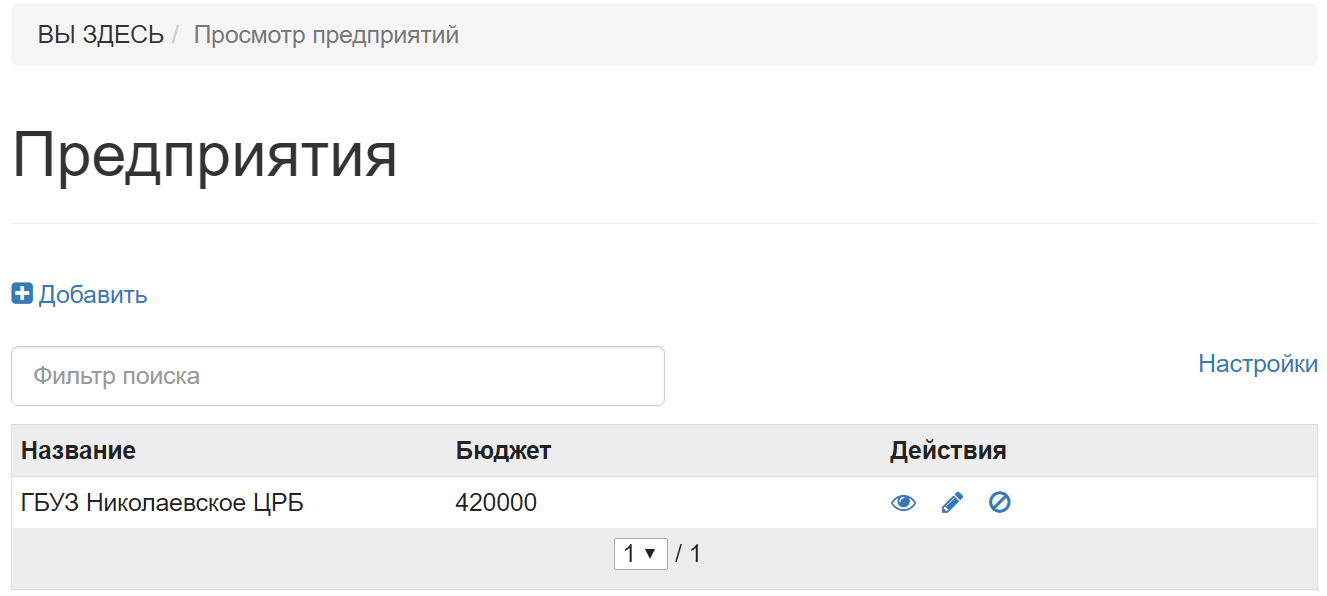
\includegraphics[scale=0.5]{screen_companies}
\caption{Все доступные пользователю предприятия}
\label{fig:screen_companies}
\end{figure}

\begin{figure}[H]
\centering
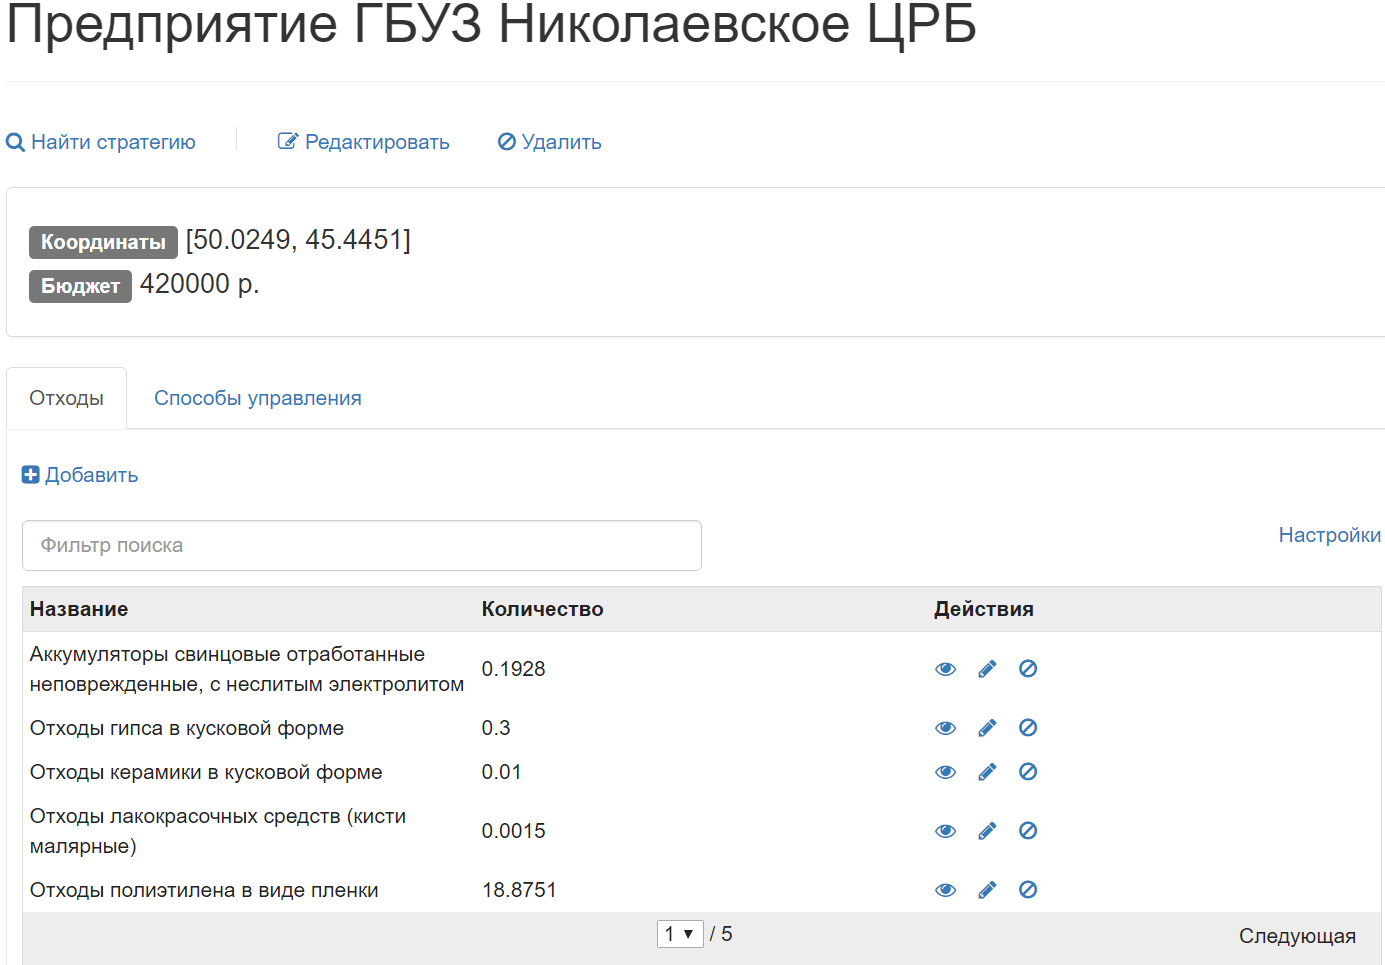
\includegraphics[scale=0.5]{screen_company}
\caption{Профиль предприятия}
\label{fig:screen_company}
\end{figure}

\section{Добавление отходов для предприятия}

\ttl

\subsection{Наименование операции}

Полное наименование операции «Добавление отходов для предприятия».

\subsection{Условия выполнения операции}

Операция выполняется только если пользователю принадлежит предприятие, для которого добавляются отходы.

\subsection{Основные действия}

Необходимо в профиле предприятия в разделе «Отходы» щелкнуть на кнопку «Добавить». Далее, введя данные, нажать кнопку «Создать». На рисунке~\ref{fig:screen_create_waste} показана форма создания отходов для предприятия.

\begin{figure}[H]
\centering
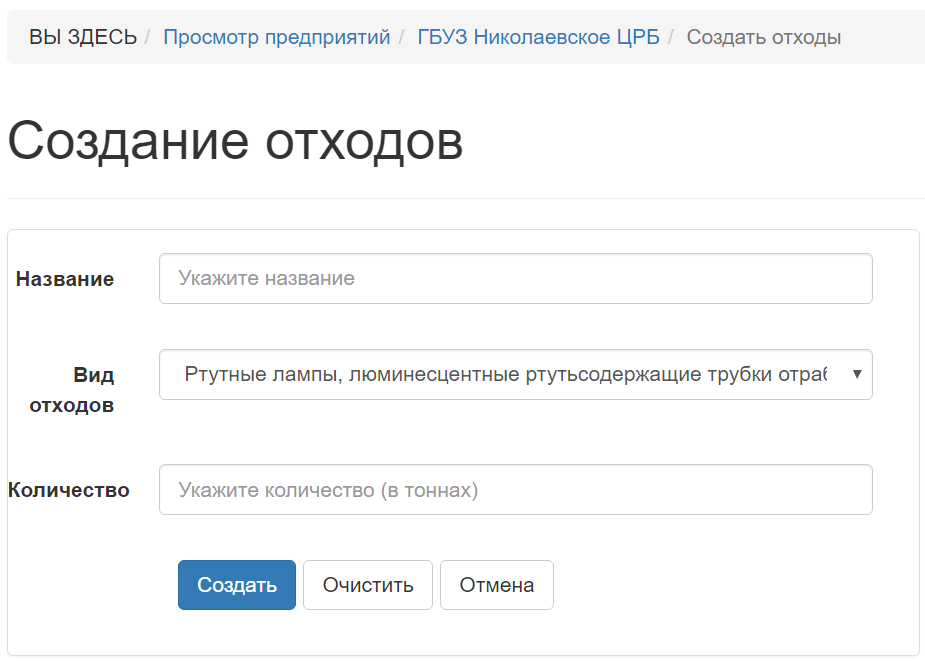
\includegraphics[scale=0.5]{screen_create_waste}
\caption{Форма создания отходов}
\label{fig:screen_create_waste}
\end{figure}

\section{Изменение отходов предприятия}

\ttl

\subsection{Наименование операции}

Полное наименование операции «Изменение отходов предприятия».

\subsection{Условия выполнения операции}

Операция выполняется только если предприятие имеет хотя бы один вид отходов.

\subsection{Основные действия}

Необходимо в профиле предприятия в разделе «Отходы» щелкнуть на иконку «карандаш» в столбце действия таблицы или тоже самое можно сделать в профиле отхода (см. рисунок~\ref{fig:screen_waste}). Далее, введя данные, нажать кнопку «Изменить». На рисунке~\ref{fig:screen_edit_waste} показана форма изменения данных об отходах предприятия.

\begin{figure}[H]
\centering
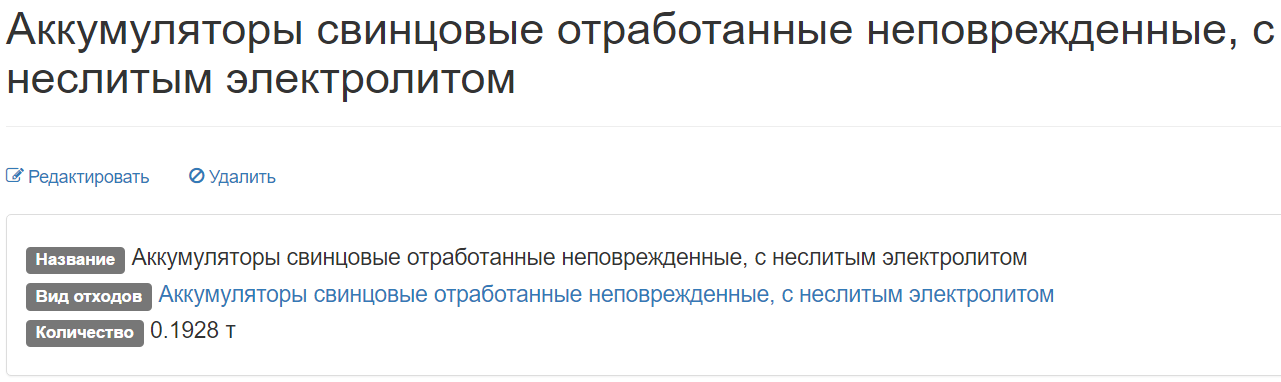
\includegraphics[scale=0.6]{screen_waste}
\caption{Профиль отходов}
\label{fig:screen_waste}
\end{figure}

\begin{figure}[H]
\centering
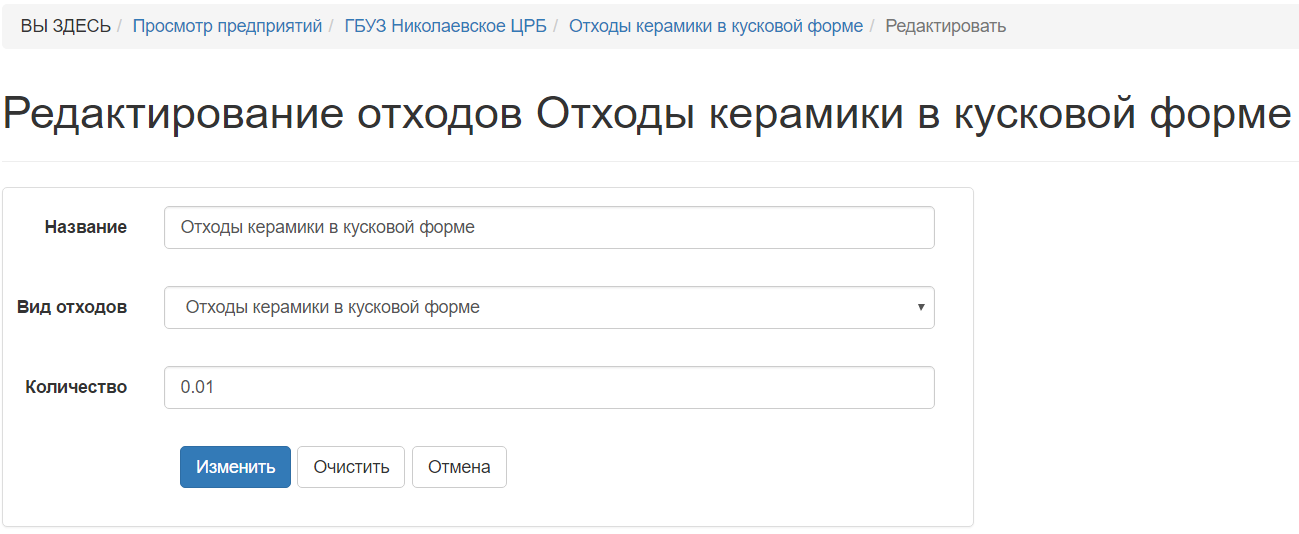
\includegraphics[scale=0.5]{screen_edit_waste}
\caption{Форма редактирования отходов}
\label{fig:screen_edit_waste}
\end{figure}

\section{Удаление отходов предприятия}

\ttl

\subsection{Наименование операции}

Полное наименование операции «Удаление отходов предприятия».

\subsection{Условия выполнения операции}

Операция выполняется только если предприятие имеет хотя бы один вид отходов.

\subsection{Основные действия}

Необходимо в профиле предприятия в разделе «Отходы» щелкнуть на иконку «запрет» в столбце действия таблицы или тоже самое можно сделать в профиле отхода.

\section{Добавление способа управления отходами для предприятия}

\ttl

\subsection{Наименование операции}

Полное наименование операции «Добавление способа управления отходами для предприятия».

\subsection{Условия выполнения операции}

Операция выполняется только если пользователю принадлежит предприятие, для которого добавляется способ управления отходами.

\subsection{Основные действия}

Необходимо в профиле предприятия в разделе «Способы управления» щелкнуть на кнопку «Добавить». Далее, введя данные, нажать кнопку «Создать». На рисунке~\ref{fig:screen_create_method} показана форма создания способа управления отходами для предприятия.

\begin{figure}[H]
\centering
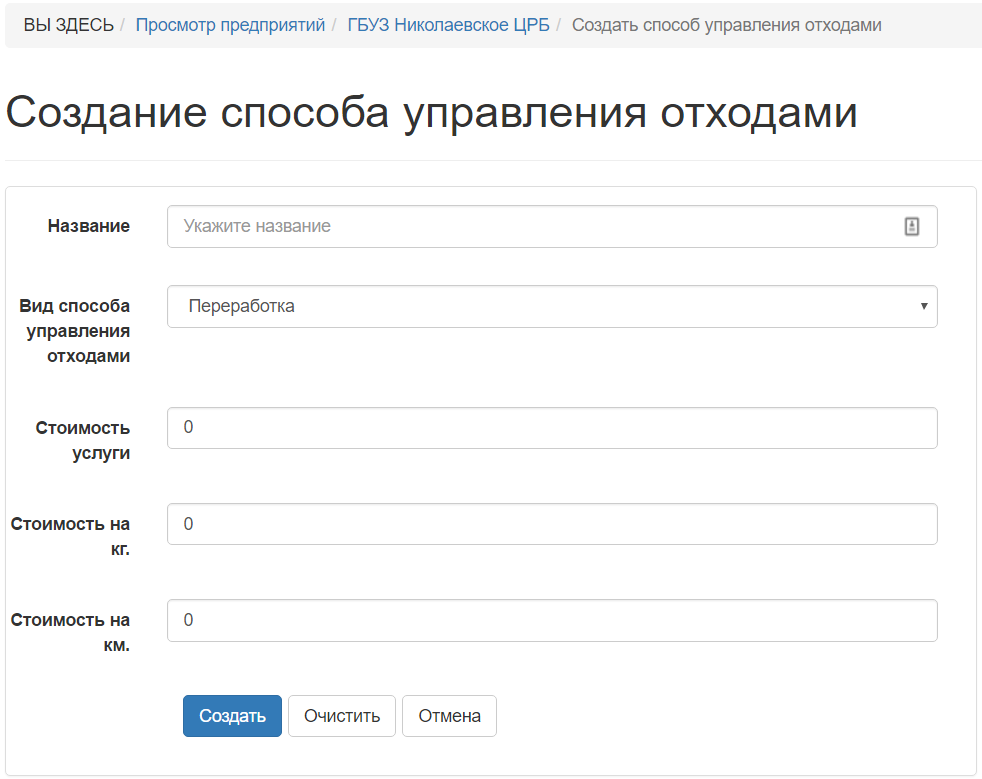
\includegraphics[scale=0.6]{screen_create_method}
\caption{Форма создания способа управления отходами}
\label{fig:screen_create_method}
\end{figure}

\section{Изменение способа управления отходами предприятия}

\ttl

\subsection{Наименование операции}

Полное наименование операции «Изменение способа управления отходами предприятия».

\subsection{Условия выполнения операции}

Операция выполняется только если предприятие имеет хотя бы один способ управления отходами.

\subsection{Основные действия}

Необходимо в профиле предприятия в разделе «Способы управления» щелкнуть на иконку «карандаш» в столбце действия таблицы или тоже самое можно сделать в профиле способа управления отходами. Далее, введя данные, нажать кнопку «Изменить». На рисунке~\ref{fig:screen_edit_method} показана форма изменения данных о способе управления отходами предприятия.

\begin{figure}[H]
\centering
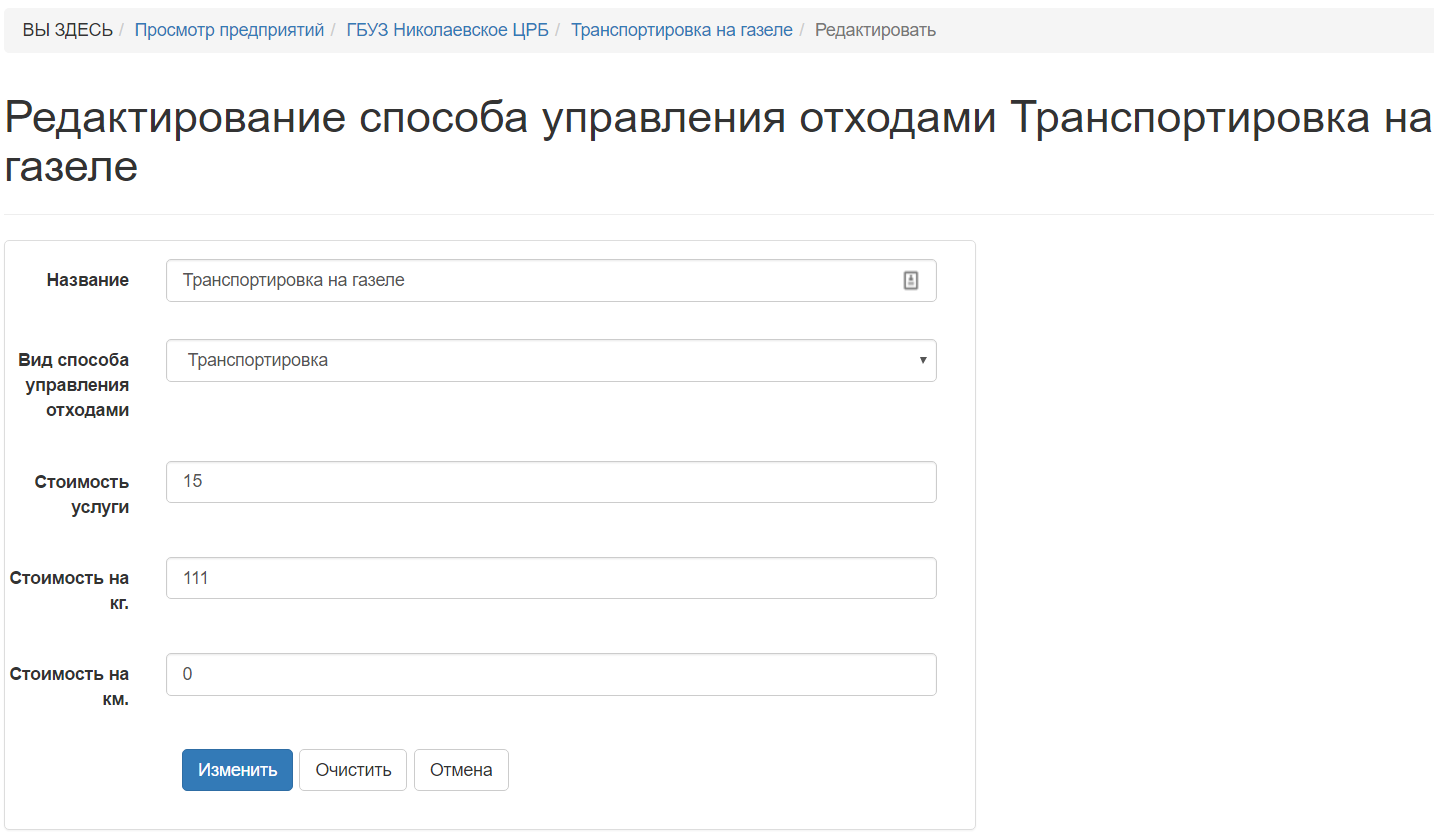
\includegraphics[scale=0.5]{screen_edit_method}
\caption{Форма редактирования способа управления отходами}
\label{fig:screen_edit_method}
\end{figure}

\section{Удаление способа управления отходами предприятия}

\ttl

\subsection{Наименование операции}

Полное наименование операции «Удаление способа управления отходами предприятия».

\subsection{Условия выполнения операции}

Операция выполняется только если предприятие имеет хотя бы один способ управления отходами.

\subsection{Основные действия}

Необходимо в профиле предприятия в разделе «Способы управления» щелкнуть на иконку «запрет» в столбце действия таблицы или тоже самое можно сделать в профиле способа управления отходами.

\section{Создание предприятия}

\ttl

\subsection{Наименование операции}

Полное наименование операции «Создание предприятия».

\subsection{Условия выполнения операции}

Операция может быть выполнена в любой момент работы системы.

\subsection{Основные действия}

Необходимо в меню выбрать пункт -- «Создать», далее «Предприятие». Затем, введя данные, нажать кнопку «Создать». На рисунке~\ref{fig:screen_create_company} показана форма создания предприятия.

\begin{figure}[H]
\centering
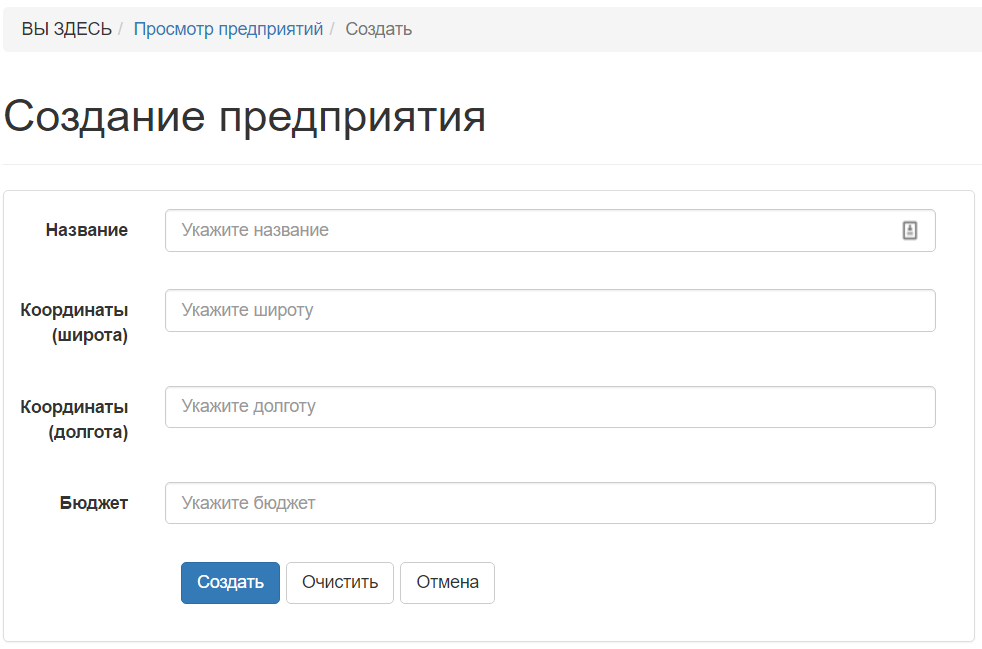
\includegraphics[scale=0.6]{screen_create_company}
\caption{Форма создания предприятия}
\label{fig:screen_create_company}
\end{figure}

\section{Изменение предприятия}

\ttl

\subsection{Наименование операции}

Полное наименование операции «Изменение предприятия».

\subsection{Условия выполнения операции}

Операция выполняется только если пользователь имеет хотя бы одно предприятие.

\subsection{Основные действия}

Необходимо в профиле предприятия щелкнуть на иконку «карандаша» или тоже самое сделать в разделе всех предприятий пользователя. Затем, введя данные, нажать кнопку «Изменить». На рисунке~\ref{fig:screen_edit_company} показана форма редактирования предприятия.

\begin{figure}[H]
\centering
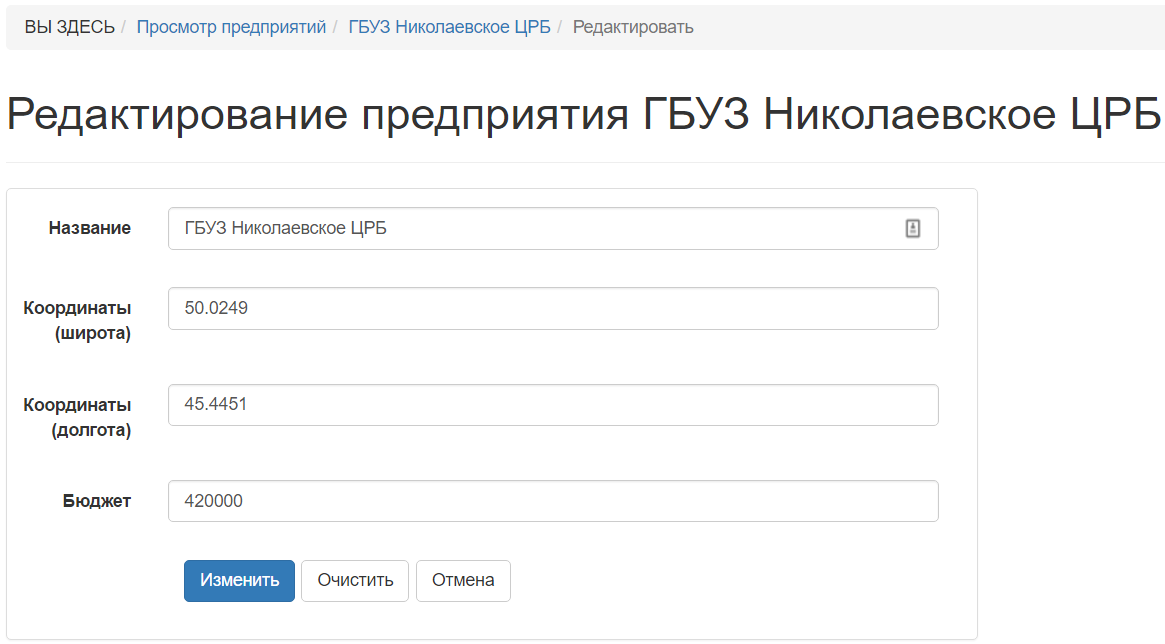
\includegraphics[scale=0.6]{screen_edit_company}
\caption{Форма редактирования предприятия}
\label{fig:screen_edit_company}
\end{figure}

\section{Удаление предприятия}

\ttl

\subsection{Наименование операции}

Полное наименование операции «Удаление предприятия».

\subsection{Условия выполнения операции}

Операция выполняется только если пользователь имеет хотя бы одно предприятие.

\subsection{Основные действия}

Необходимо в списке всех предприятий щелкнуть на иконку «запрет» в столбце действия таблицы или тоже самое можно сделать в профиле предприятия.

\section{Поиск стратегии управления отходами предприятия}

\ttl

\subsection{Наименование операции}

Полное наименование операции «Поиск стратегии управления отходами предприятия».

\subsection{Условия выполнения операции}

Операция выполняется только если пользователь имеет хотя бы одно предприятие, обладающее отходами.

\subsection{Основные действия}

Необходимо в профиле предприятия необходимо нажать на кнопку «Найти стратегию». После некоторого времени ожидания, на появившемся модальном окне, система отобразить сгенерированную стратегию управления отходами предприятия (см. рисунки~\ref{fig:screen_strategy_1} и~\ref{fig:screen_strategy_3}).

\begin{figure}[H]
\centering
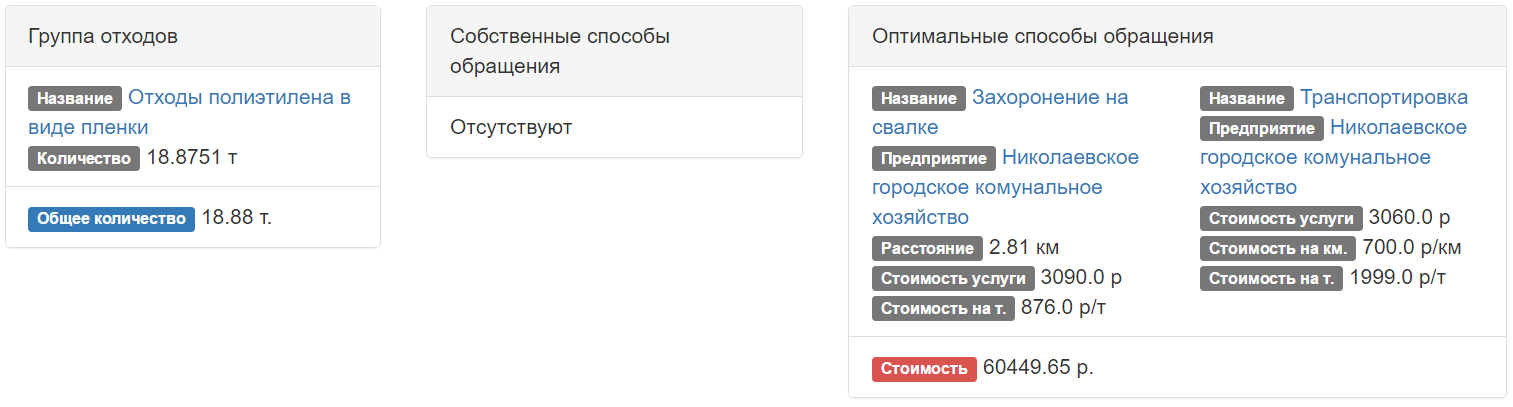
\includegraphics[scale=0.51]{screen_strategy_1}
\caption{Форма отображения сгенерированной стратегии управления отходами в системе (фрагмент 1)}
\label{fig:screen_strategy_1}
\end{figure}

\begin{figure}[H]
\centering
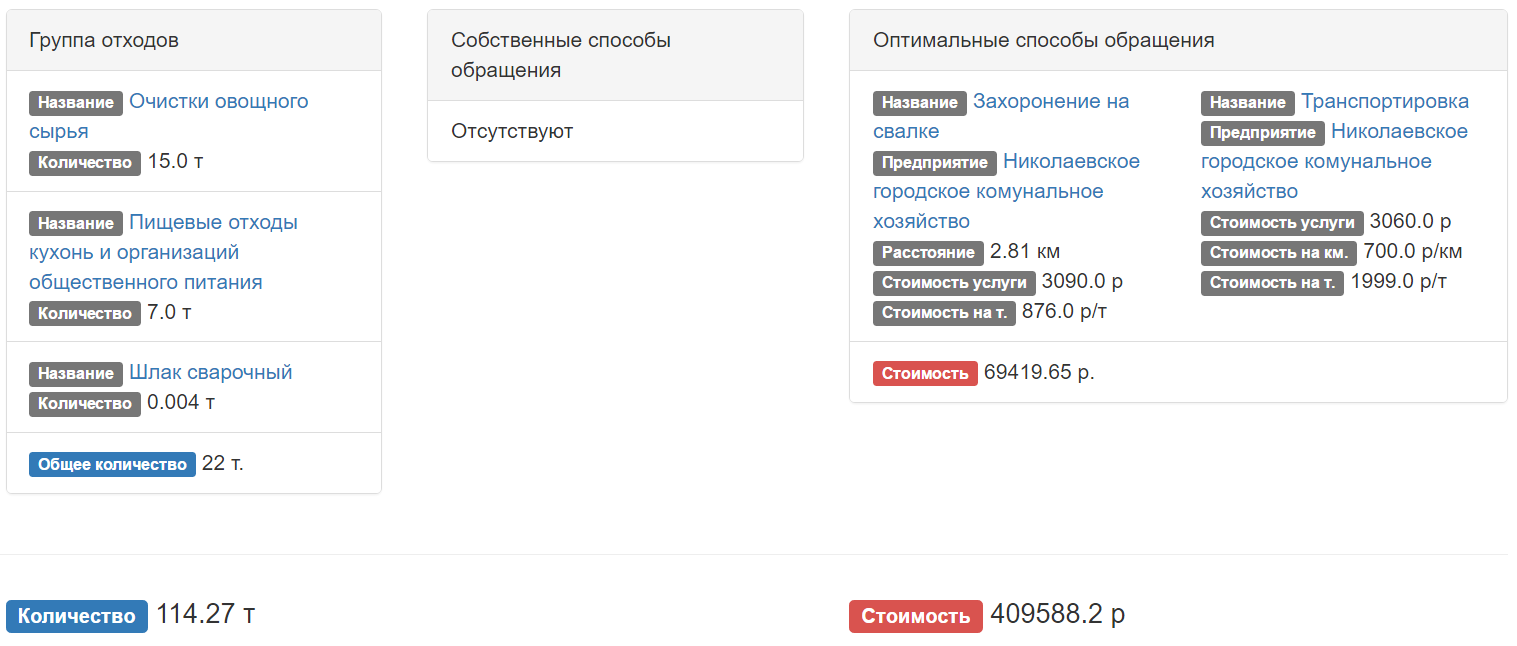
\includegraphics[scale=0.51]{screen_strategy_3}
\caption{Форма отображения сгенерированной стратегии управления отходами в системе (фрагмент 2)}
\label{fig:screen_strategy_3}
\end{figure}

\chapter{Аварийные ситуации}

\ttl

\section{Действия при длительных отказах технических средств}\label{sec:otkaz_sec}

В случае длительных отказов технических средств необходимо проверку оборудования в специализированном центре, после чего произвести заново установку программного обеспечения, в соответствии с руководством системного программиста.

\section{Действия по восстановлению программ и данных при отказе магнитных носителей или обнаружении ошибок в данных}

При отказе магнитных носителей или обнаружении ошибок в данных необходимо произвести восстановление файла проекта и файлов исходных кодов, используемых в проекте. Если данные действия не приведут к желаемому результату, нужно действовать в соответствии с пунктом~\ref{sec:otkaz_sec} данного руководства.

\end{document}